\documentclass[12pt, a4paper, titlepage]{article}
\usepackage[ngerman]{babel}      % Deutsche Sprachunterstützung
\usepackage[utf8]{inputenc}      % Umlaute und Sonderzeichen
\usepackage{graphicx}            % Für Grafiken
\usepackage{amsmath, amssymb}   % Für erweiterte Mathematikumgebungen
\usepackage{caption}             % Für Bildunterschriften
\usepackage{float}
\usepackage{booktabs}
\usepackage{array}
\usepackage[table]{xcolor}
\usepackage{hhline}


% Deckblatt
\title{Ausarbeitung MS01: Messungen mit einem Oszilloskop}
\author{Gruppe D \\ Marie Schmalz, Laurenz Wrobel, Phil Reinartz}
\date{\today}

\begin{document}

\maketitle % Erzeugt das Deckblatt mit Titel, Autor und Datum
\tableofcontents
\newpage

\section{Einleitung}
Es folgt die Umsetzung der in dem Versuch geforderten Punkte für die Ausarbeitung.

\newpage


\section{Oszillogramme}


\begin{figure}[H]
  \centering
  \begin{minipage}[t]{0.48\textwidth}
    \centering
    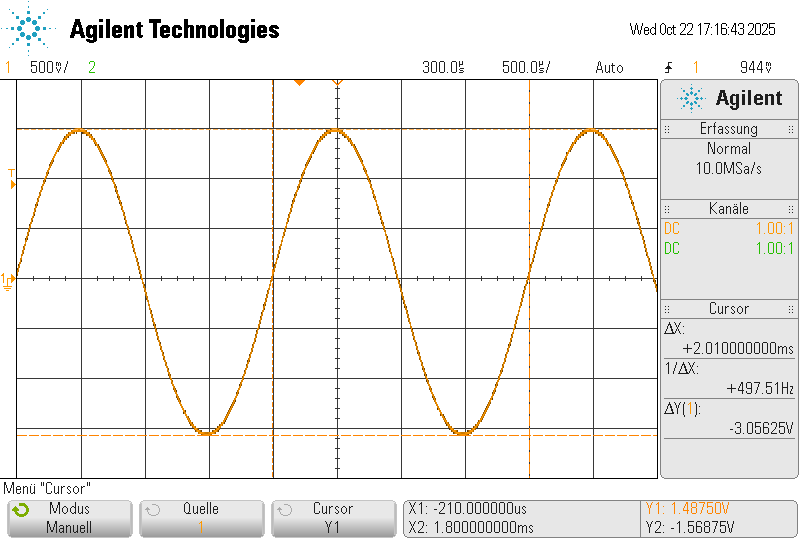
\includegraphics[width=\textwidth]{scope_0.png}
    \caption{Manuelle Ermittlung von (T, $U_{ss}$) für eine Sinusspannung.}
  \end{minipage}%
  \hfill
  \begin{minipage}[t]{0.48\textwidth}
    \centering
    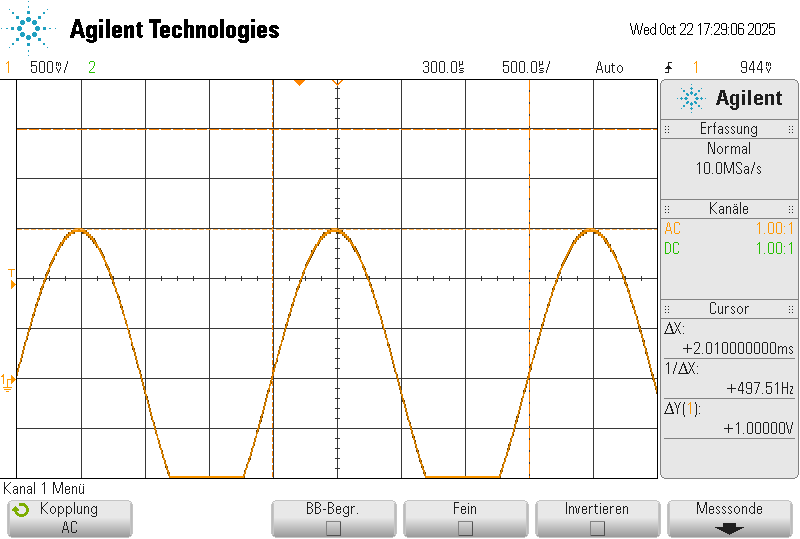
\includegraphics[width=\textwidth]{scope_1.png}
    \caption{Manuelle Ermittlung des Gleichspannungsanteils einer Sinusspannung (Mischsignal).}
  \end{minipage}
\end{figure}

\begin{figure}[H]
  \centering
  \begin{minipage}[t]{0.48\textwidth}
    \centering
    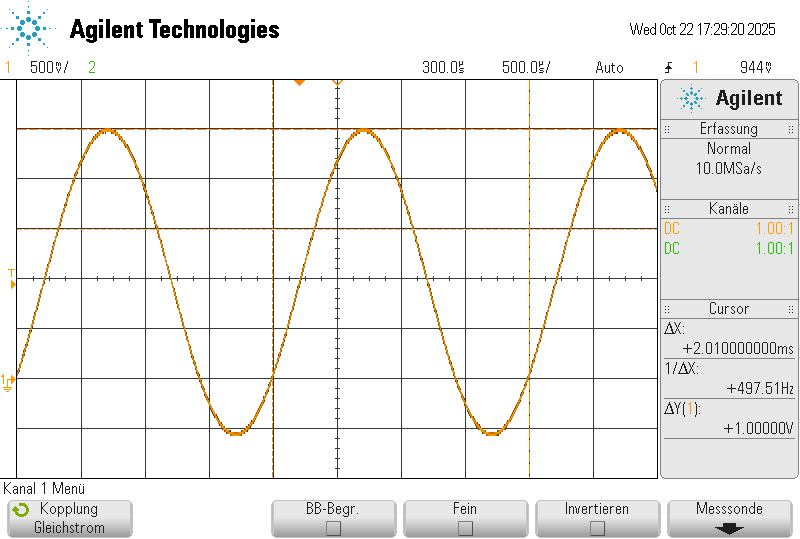
\includegraphics[width=\textwidth]{scope_2.png}
    \caption{Manuelle Ermittlung des Gleichspannungsanteils einer Sinusspannung (Mischsignal).}
  \end{minipage}%
  \hfill
  \begin{minipage}[t]{0.48\textwidth}
    \centering
    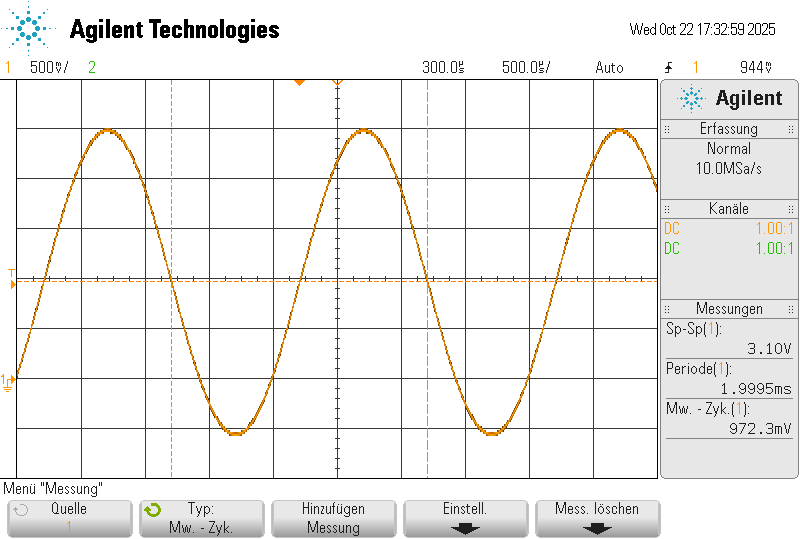
\includegraphics[width=\textwidth]{scope_3.png}
    \caption{Ermittlung von ($U_{ss}$, T, $\overline{U}$) für eine Sinusspannung.}
  \end{minipage}
\end{figure}

\begin{figure}[H]
  \centering
  \begin{minipage}[t]{0.48\textwidth}
    \centering
    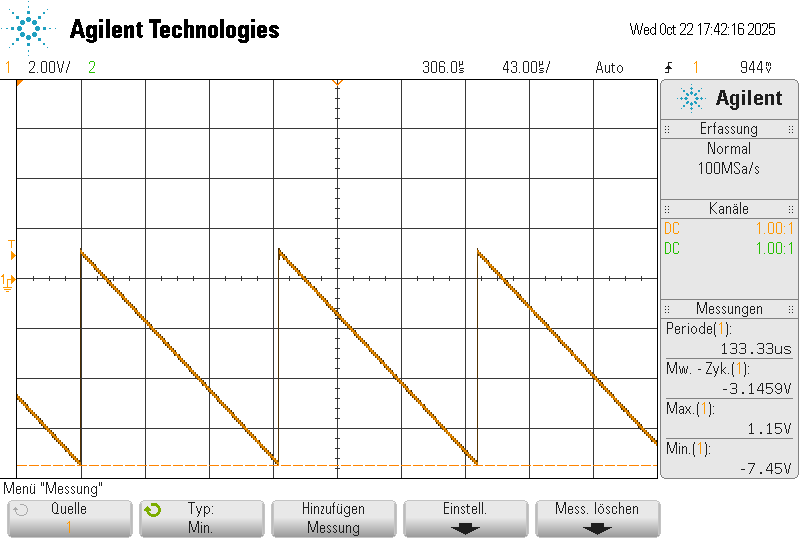
\includegraphics[width=\textwidth]{scope_5.png}
    \caption{Ermittlung von (T, $\overline{U}$, $U_{Max}$, $U_{Min}$) für eine Sägezahnspannung.}
  \end{minipage}%
  \hfill
  \begin{minipage}[t]{0.48\textwidth}
    \centering
    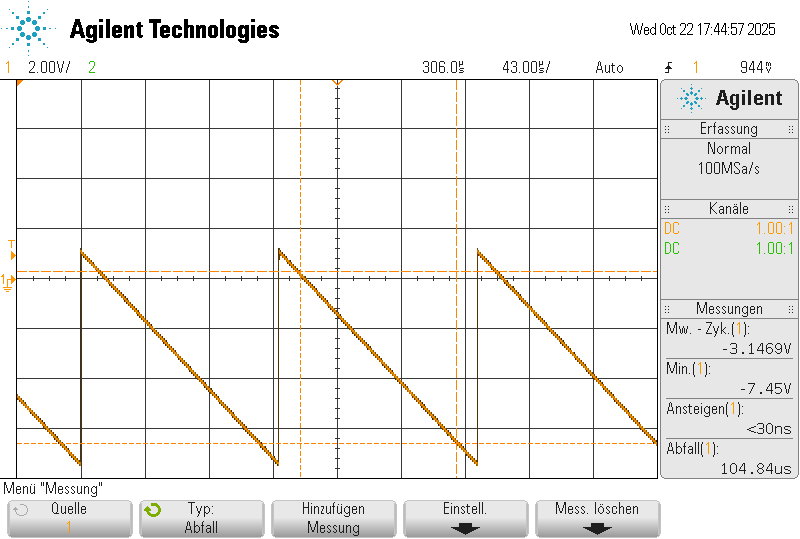
\includegraphics[width=\textwidth]{scope_6.png}
    \caption{Ermittlung von ($t_{r}$, $t_{f}$) für eine Sägezahnspannung.}
  \end{minipage}
\end{figure}

\begin{figure}[H]
  \centering
  \begin{minipage}[t]{0.48\textwidth}
    \centering
    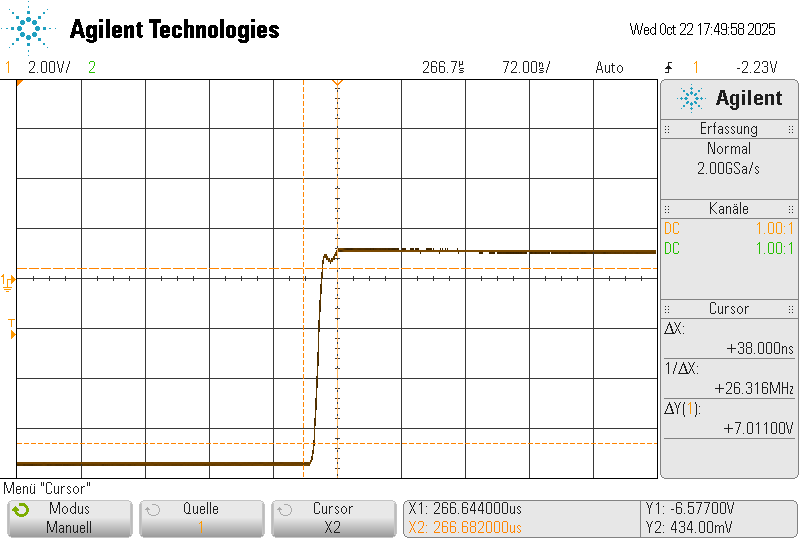
\includegraphics[width=\textwidth]{scope_7.png}
    \caption{Manuelle Ermittlung von $t_{r}$ für eine Sägezahnspannung.}
  \end{minipage}%
  \hfill
  \begin{minipage}[t]{0.48\textwidth}
    \centering
    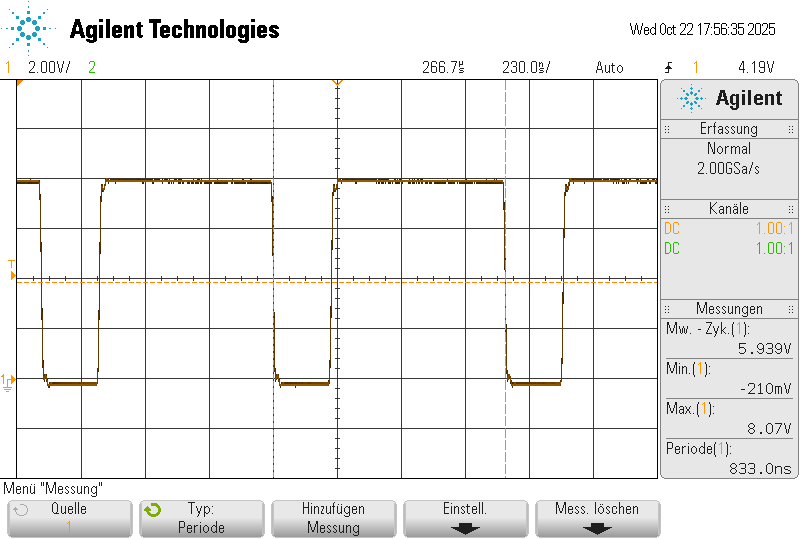
\includegraphics[width=\textwidth]{scope_8.png}
    \caption{Ermittlung von (T, $\overline{U}$, $U_{Max}$, $U_{Min}$) für eine Rechteckspannung.}
  \end{minipage}
\end{figure}

\begin{figure}[H]
  \centering
  \begin{minipage}[t]{0.48\textwidth}
    \centering
    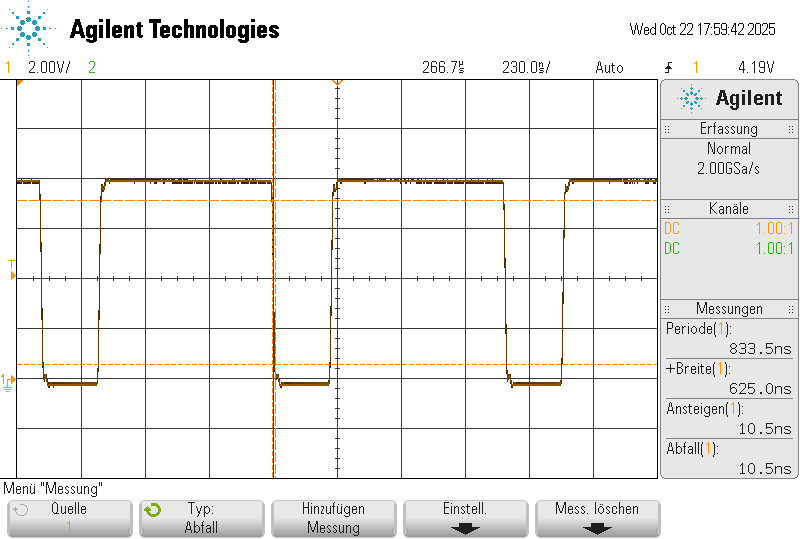
\includegraphics[width=\textwidth]{scope_9.png}
    \caption{Ermittlung von ($t_{p}$, $t_{r}$, $t_{f}$) für eine Rechteckspannung.}
  \end{minipage}
  % Wenn ungerade Anzahl Bilder, diese Hälfte leer lassen oder zentrieren
  \hfill
  \begin{minipage}[t]{0.48\textwidth}
    % leer oder alternativ Text/Bild
  \end{minipage}
\end{figure}

\newpage

\section{Messwertetabelle}





\begin{table}[h]
	\centering
	\caption{Messwerte mit abwechselnd grauen und weißen Zeilen}
	\rowcolors{2}{gray!15}{white} % Start bei 2. Zeile: grau, dann weiß usw.
	\setlength{\arrayrulewidth}{0.75pt}	 
	\resizebox{\textwidth}{!}{%
	\begin{tabular}{>{\bfseries}l|c|c|c|c|c|c|c|c} % l für left c für center, | für strich
    
		\textbf{Signalformen} & $\overline{\mathbf{U}}$ [V]  & $\mathbf{U}_{\mathbf{ss}}$ [V]  & \textbf{T} [s] & $\mathbf{u}_{\mathbf{max}}$ [V]
		& $\mathbf{u}_{\mathbf{min}}$ [V] & $\mathbf{t}_{\mathbf{r}}$ [s]   & $\mathbf{t}_{\mathbf{f}}$ [s] &  $\mathbf{t}_{\mathbf{p}}$ [s] \\
		\hhline{|--------|}
		\textbf{Sinus} & 0.97 & 3.1 & 2.01m & /  & /  & /  & / & /  \\
		\textbf{Sägezahn} & -3.15 & / & 133.33$\mu$ & 1.15  & -7.45  & $<30$n  & 104.84$\mu$ & /  \\
		\textbf{Rechteck} & 5.94  & /  & 833n  & 8.07  & -210m  & 10.5n  & 10.5n  & 625.0n  \\
    		
  	\end{tabular}
	}
\end{table}

\newpage

\section{Vorteile von Digitalen Speicheroszilloskopen}






\end{document}


